\documentclass{beamer}

\usepackage{ucs}
\usepackage{amsfonts,amsmath}
\usepackage[utf8x]{inputenc}
\usepackage[protrusion=true,expansion=true]{microtype}
\usepackage{setspace}
\usepackage{pdfsync}
\usepackage{tikz}
\usepackage{macros}
\usepackage{mathpartir}

\usetikzlibrary{automata, positioning, shapes.geometric, shapes.misc,
  chains, backgrounds, fit, decorations.pathmorphing}

\tikzset{
  state/.style={
    rounded rectangle,
    very thick,draw=black!50,
    top color=white, bottom color=black!20,
    minimum size=2em,
    text height=1.5ex,text depth=.25ex
  }
}

\tikzset{
  tribox/.style={
    isosceles triangle,
    isosceles triangle apex angle=40,
  }
}

\setbeamertemplate{footline}[frame number]
\setbeamertemplate{navigation symbols}{}
\setbeamertemplate{itemize item}[circle]

\usefonttheme{serif}
\usecolortheme[rgb={0.7,0.2,0.2}]{structure}
\definecolor{greenish}{rgb}{0.20,0.48,0.09} % vert des exemples


\date{\small June 20, 2012\\[0.5em]
  \scriptsize PPS -- Groupe de travail théorie des types et
  réalisabilité
}

\title{Certificates for incremental type checking}

\author[Matthias Puech \& Yann Régis-Gianas] {
  Matthias Puech\inst{1,2} \and Yann Régis-Gianas\inst{2}
}

\institute {
  \inst 1 {Dept. of Computer Science, University of Bologna} \and
  \inst 2 {Univ. Paris Diderot, Sorbonne Paris Cité, PPS, CNRS,  ${\pi}r^2$, INRIA}
}

\begin{document}

\frame\titlepage

\subsection{How to make a type checker incremental?}

\begin{frame}
  \begin{center}
    \large
    {\bf Problem 1:}
    How to make a type checker incremental?
  \end{center}
\end{frame}

\begin{frame}{\textcolor{gray}{Certificates for incremental} type-checking}

  \begin{block}{Observations}
    \begin{itemize}
    \item Program elaboration is more and more an \emph{interaction}
      between the programmer and the type-checker
    \item The richer the type system is, the more expensive
      type-checking gets
    \end{itemize}
    \begin{example}
      \begin{itemize}
      \item type inference (\eg\ \sysname{Haskell}, unification)
      \item dependent types (conversion, esp. reflection)
      \item very large term
      \end{itemize}
    \end{example}
  \end{block}
  \pause
  \begin{center}
    \large \emph{\ldots but is called repeatedly with \emph{almost} the same input}
  \end{center}
\end{frame}

\begin{frame}{\textcolor{gray}{Certificates for incremental}
    type-checking}
  \vspace{0.5em}
  \begin{center}
    \only<1>{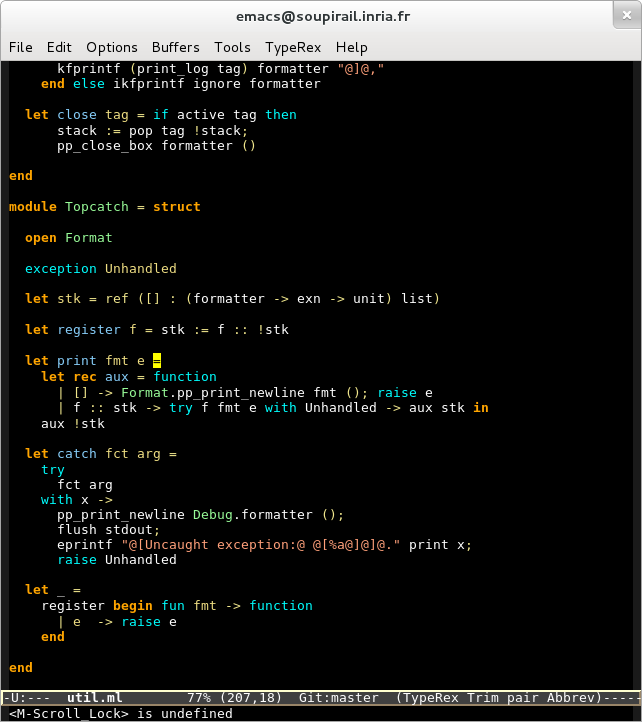
\includegraphics[height=0.9\textheight]{images/emacs1.png}}%
    \only<2>{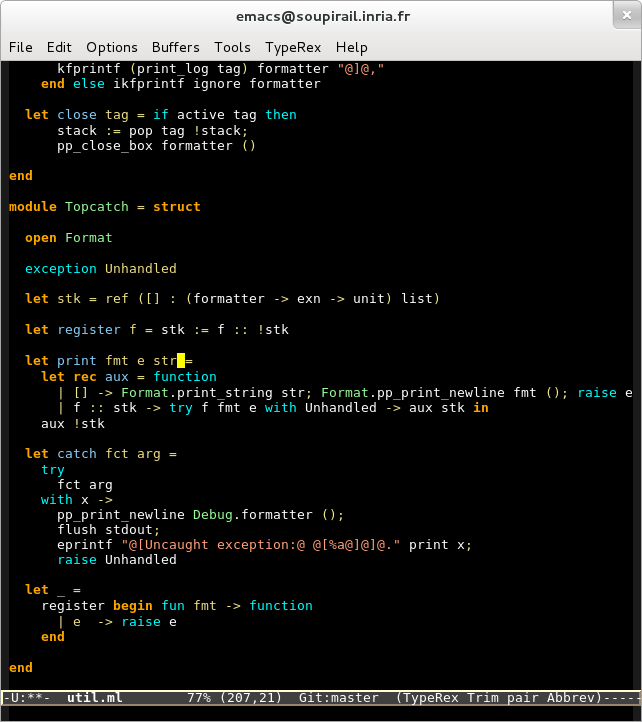
\includegraphics[height=0.9\textheight]{images/emacs2.png}}%
    \only<3>{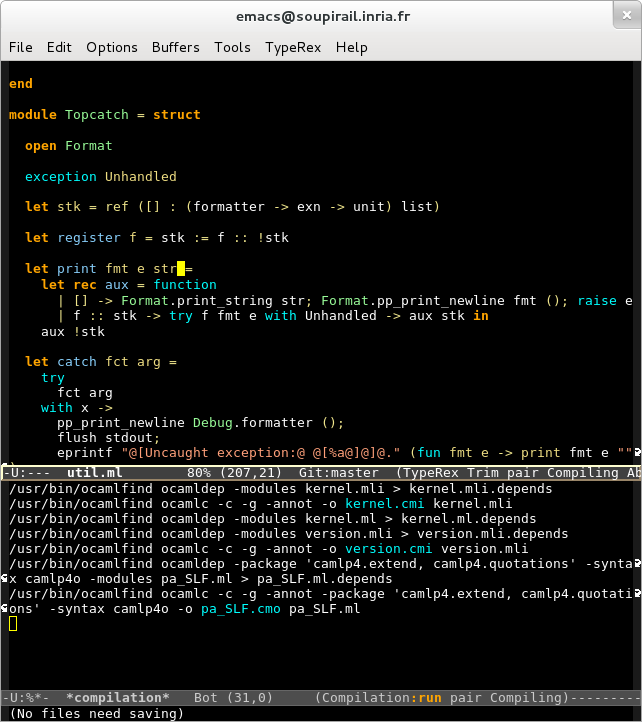
\includegraphics[height=0.9\textheight]{images/emacs3.png}}%
    \only<4>{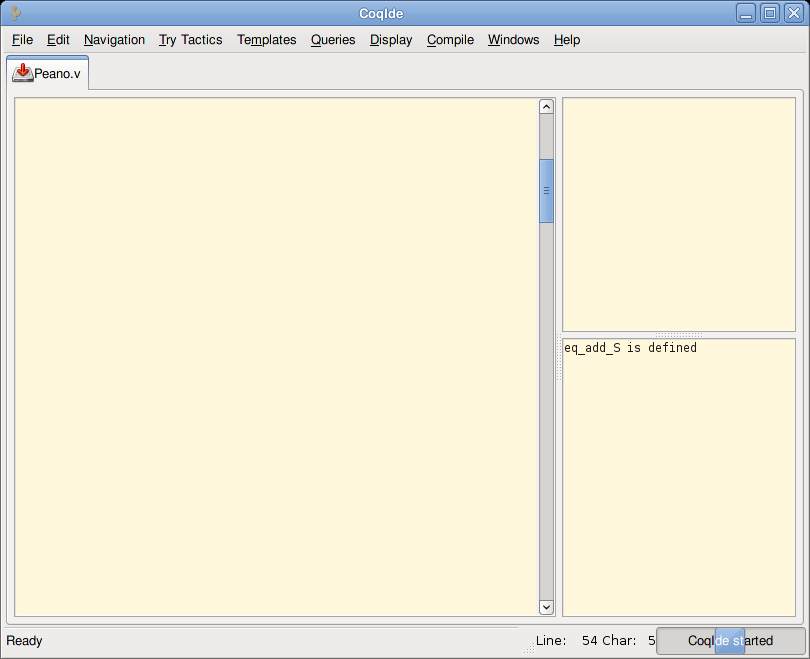
\includegraphics[width=0.85\textwidth]{images/coqide00.png}}%
    \only<5>{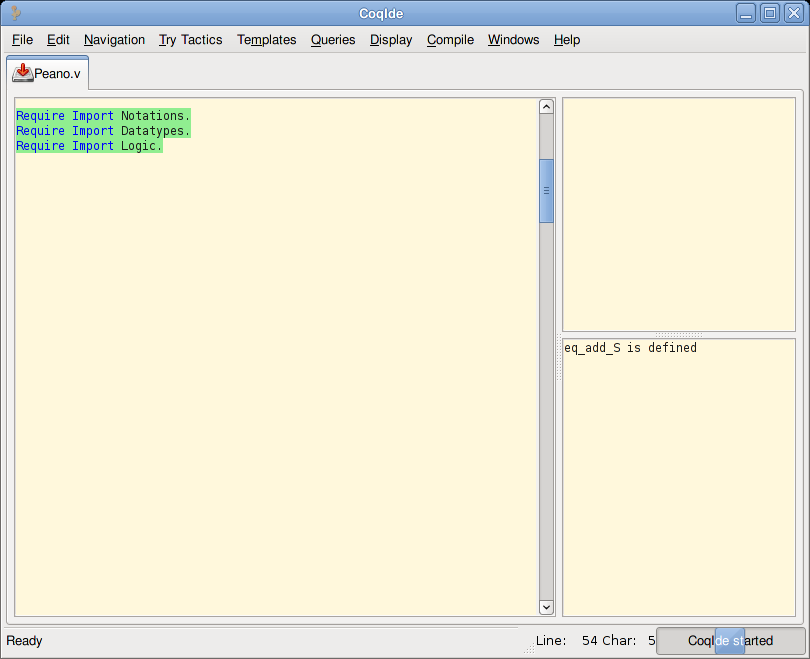
\includegraphics[width=0.85\textwidth]{images/coqide0.png}}%
    \only<6>{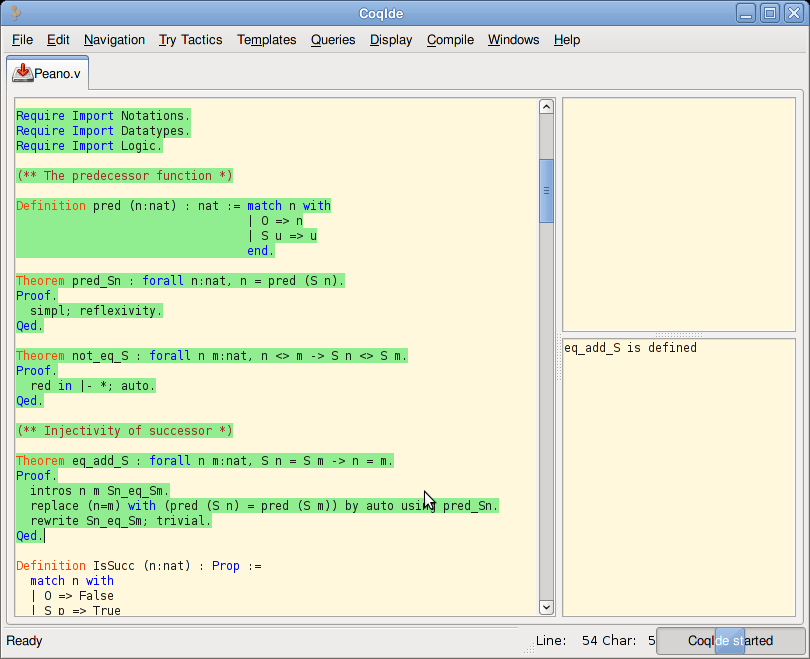
\includegraphics[width=0.85\textwidth]{images/coqide.png}}%
    \only<7>{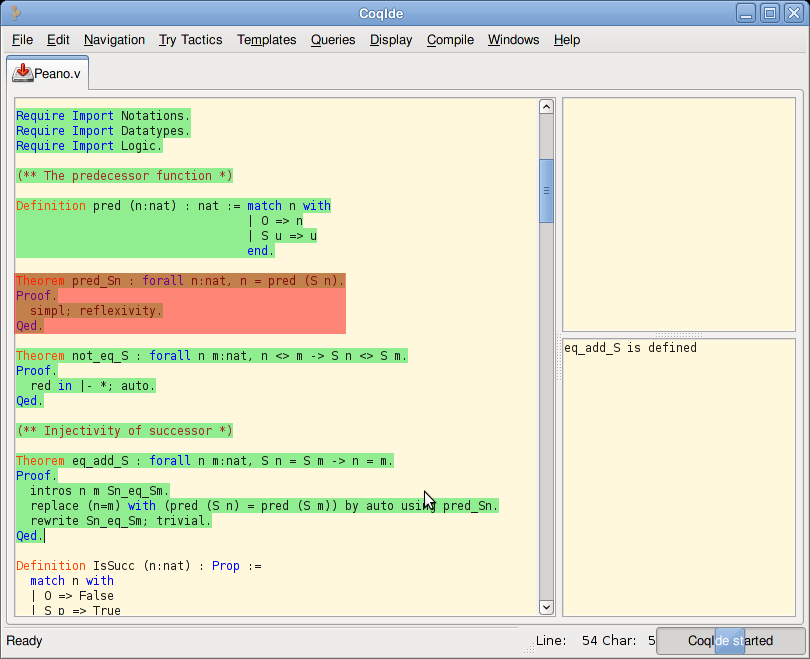
\includegraphics[width=0.85\textwidth]{images/coqide2.png}}%
    \only<8>{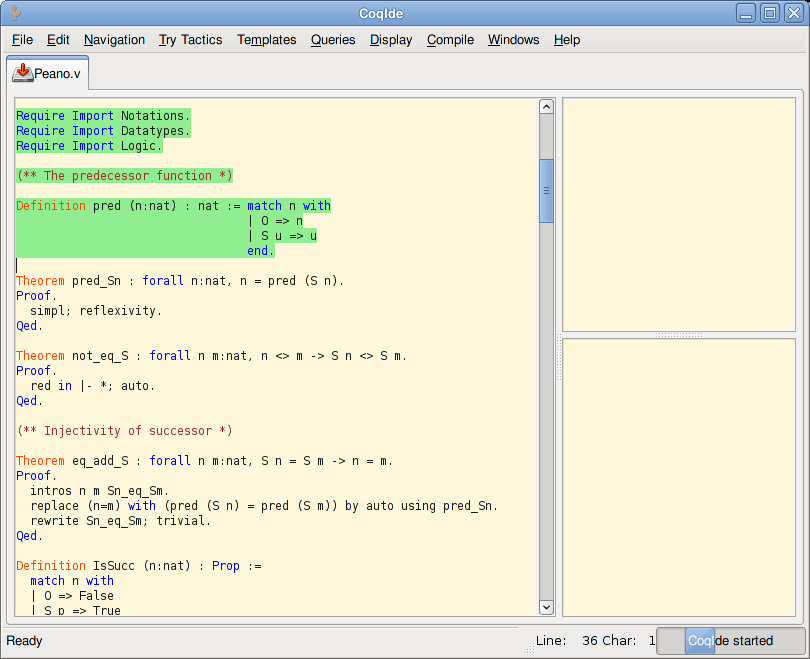
\includegraphics[width=0.85\textwidth]{images/coqide4.png}}%
    \only<9>{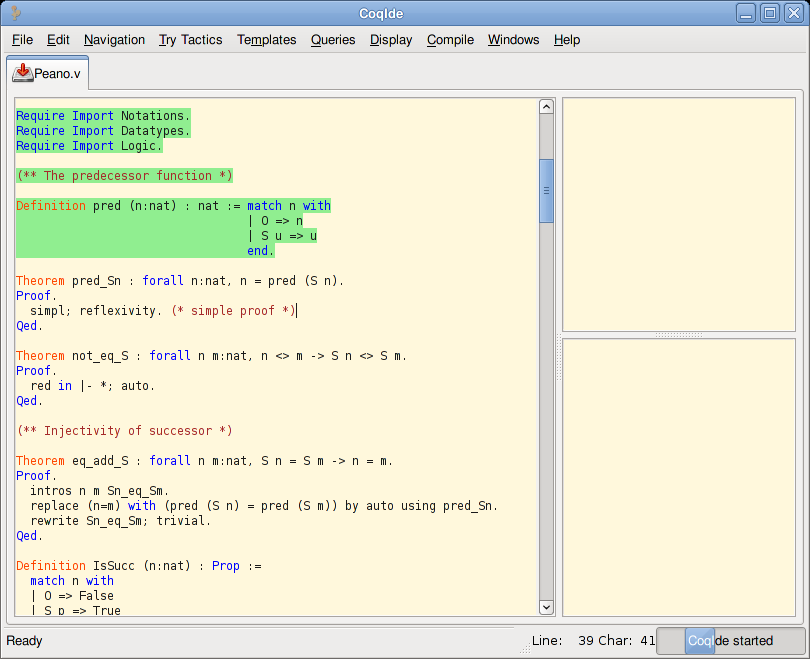
\includegraphics[width=0.85\textwidth]{images/coqide5.png}}%
    \only<10>{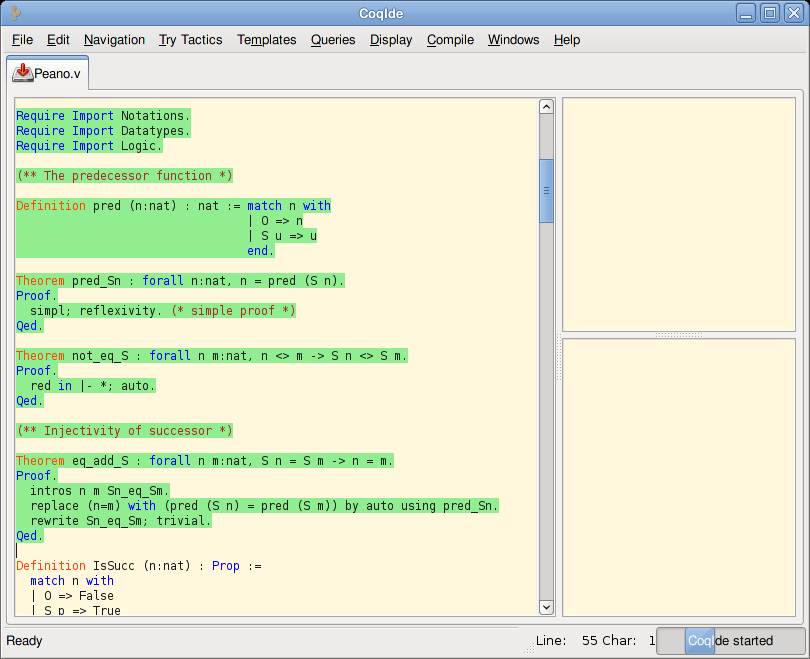
\includegraphics[width=0.85\textwidth]{images/coqide6.png}}%
    \only<11>{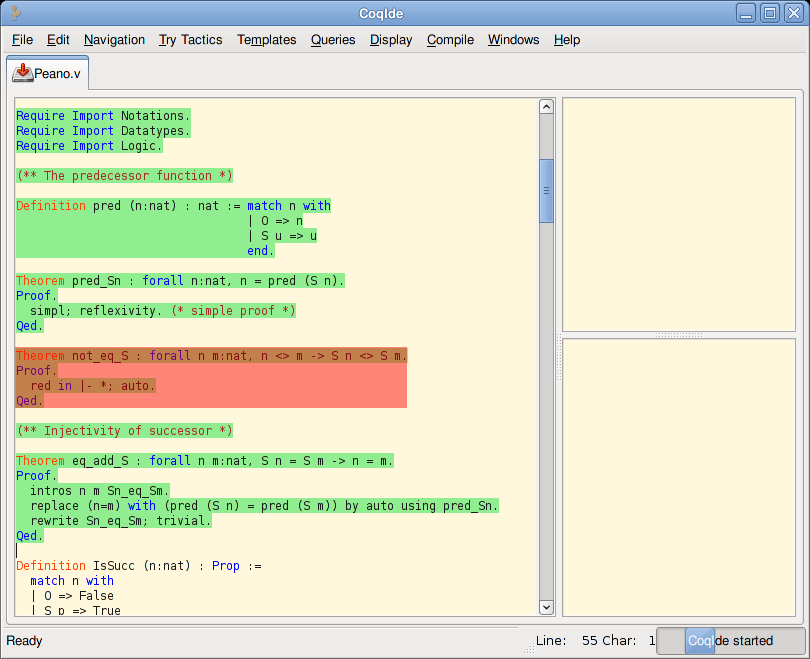
\includegraphics[width=0.85\textwidth]{images/coqide7.png}}%
  \end{center}
\end{frame}


\begin{frame}{\textcolor{gray}{Certificates for} incremental
    \textcolor{gray}{type checking}}

    \begin{block}{Problem}
      \emph{How to take advantage of the knowledge from previous type-checks?}
      \begin{itemize}
      \item Reuse already-computed results
      \item Recheck only the changed part of a program and its
        \emph{impact}
      \end{itemize}
    \end{block}
\end{frame}

\subsection{How to trust your type checker?}

\begin{frame}
  \begin{center}
    \large
    {\bf Problem 2:}
    How to trust your type checker?
  \end{center}
\end{frame}

\begin{frame}{A compiler designer's job}
  \begin{center}
    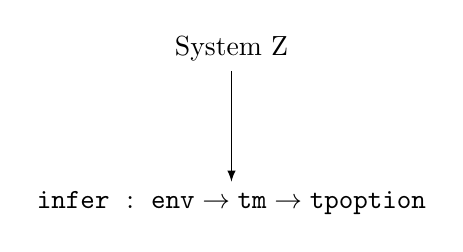
\begin{tikzpicture}[auto, >=latex]
      \node (ts) {System \sysname{Z}};

      \node (tc) [below=4em of ts] {$\tt \fct{infer}\ :\ \cst{env} \to \cst{tm} \to \app
        {\cst{tp}} \cst{option}$};

      \path[->] (ts) edge (tc);
    \end{tikzpicture}

    \vspace{2em}
    set of declarative inference rules $\to$ decision algorithm
  \end{center}
  \pause
  \begin{itemize}
  \item non trivial (inference, conversion\ldots)
  \item non compositional
  \end{itemize}

\end{frame}

\begin{frame}{\textcolor{greenish}{Example:} System \sysname{T}$_{<:}$}
  \begin{block}{Syntax}
    \vspace{-2em}
    \begin{align*}
      M &\gequal \z \gor \s M \gor M M \gor \lam x M \gor
      \recb M N x y P \\
      A &\gequal \nat \gor \even \gor \odd \gor A \to A
    \end{align*}
  \end{block}
  \begin{block}{Typing rules}
    \vspace{-2em}
    \begin{mathpar}
      \infer{\jts M \nat \and \jts N A \and \infer*{}{\mbox{$
            \begin{array}{c}
              [\jts {\var x} \nat] \quad
              [\jts {\var y} A] \\[-0.3em]
              \vdots\\
              \jts P A
            \end{array}
            $}} }{\jts {\recb M N x y P} A}

      \only<2>\alert{\infer{\jts M A \and \jsub A B}{\jts M B}}

    \end{mathpar}
  \end{block}
  \pause
  \begin{center}
    {\large\it \alert{Not syntax directed!}}
  \end{center}
\end{frame}

\begin{frame}{\textcolor{greenish}{Example:} System \sysname{T}$_{<:}$}
  \begin{block}{Typing algorithm}
    \begin{overlayarea}\textwidth{8em}
      \large \only<1>{$$ \infer{\Gamma\jts M {A\to B} \and \Gamma\jts
          N A}{\Gamma\jts{\app M N} B}
    $$}

  \only<2>{$$ \infer{ \Gamma\jts M {A\to B} \and \infer*{ \Gamma\jts N
        {A'} \and \Gamma\jsub {A'} A }{ \Gamma\jts N A } }{
      \Gamma\jts{\app M N} B }
    $$}

  \only<3>{$$ \infer{ \Gamma\jts M \nat \and \Gamma\jts N A \and
      \Gamma, \var x :\nat, \var y: A\jts P A }{\jts {\recb M N x y P}
      A}
    $$}

  \only<4->{$$ \infer{ \Gamma\jts M {T_M} \and \Gamma\jsub{T_M}{\nat}
      \and \Gamma\jts N T_N
      \\
      \Gamma, \var x:\nat, \var y:T_N\jts P {T_P}
      \\
      \Gamma, \var x:\nat, \var y:T_N\sqcap T_P\jts P {T_N\sqcap T_P}
    }{ \Gamma\jts {\recb M N x y P} {T_N\sqcap T_P} }
    $$}

  \only<5>{
    \begin{itemize}
    \item Far from the declarative system
    \item Hard to prove
    \end{itemize}
  }
\end{overlayarea}
  \end{block}
\end{frame}

\begin{frame}{How to trust your typing algorithm?}
  \begin{block}{Option 1}
    Prove equivalence:
    $$
    \app{\fct{infer}}\app{\Gamma}{M}=\app{\cst{Some}} A
    \quad\text{iff}\quad
    \vdash M : A
    $$
  \end{block}
  \pause
  \begin{block}{Option 2}
    Return a System \sysname{T}$_{<:}$ derivation:
    $$
    \fct{infer}\ :\ \cst{env}\to\cst{tm}\to\cst{tp}\times\cst{deriv}
    $$
  \end{block}
\end{frame}

\begin{frame}{Observation}

  \begin{onlyenv}<1>
    Let $\md\ =\ \finfer{M}$. \\
    Let $M'$ be a slightly modified $M$. \\
    Then $\md'\ =\ \finfer{M'}$ is a slightly modified $\md$.
  \end{onlyenv}

  \begin{onlyenv}<2>
    \begin{center}
      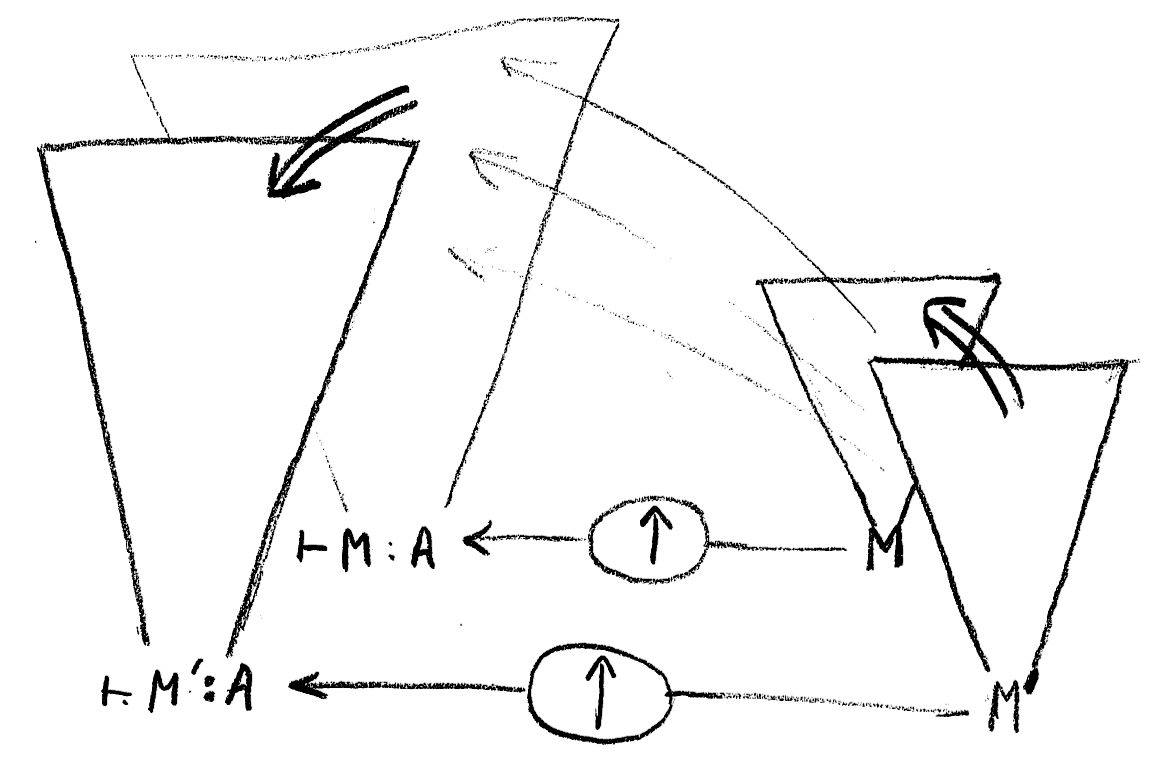
\includegraphics{images/deriv.png}
    \end{center}
  \end{onlyenv}
\end{frame}

\begin{frame}{Back to Problem 1}
  
  \begin{onlyenv}<1>
    \begin{block}{Problem}
      \emph{How to take advantage of the knowledge from previous
        type-checks?}
      \begin{itemize}
      \item Reuse pieces of a computed derivation $\md$
      \item Check only the changed part (the \emph{delta}) of a
        program $M$
      \end{itemize}

      \centering
      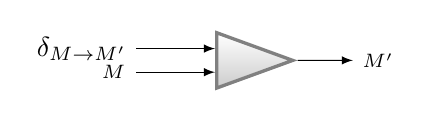
\begin{tikzpicture}[node distance=2em, >=latex, hv
        path/.style={to path={-| (\tikztotarget)}}, vh path/.style={to
          path={|- (\tikztotarget)}} ]
        \node[state, tribox] (tc) {$\finfer{}$}; \node (term)
        [left=1cm of tc.north west] {$\delta_{M\to M'}$}; \node (repo)
        [left=1cm of tc.south west] {$\md_M$}; \node (repo2) [right=of
        tc] {$\md_{M'}$};

        \path[->] (term) edge (tc.north west) (repo) edge (tc.south
        west) (tc) edge (repo2) ;
      \end{tikzpicture}
    \end{block}

    \begin{block}{Requirements}
      \begin{itemize}
      \item $\infer{\md_{M'}}{\vdash M' : A}$\quad iff\quad
        $\finfer{(\md_M, \delta_{M\to M'})} = \md_{M'}$
      \item $\finfer{(\md_M, \delta_{M\to M'})}$ computes $\md_{M'}$
        in less than $O(|M'|)$ \small\qquad\flushright (ideally
        $O(|\delta_{M\to M'}|)$)
      \end{itemize}
    \end{block}
  \end{onlyenv}

  \begin{onlyenv}<2>
    \begin{block}{Bidirectional incremental updates}
      % view the derivation as the document we're editing
      % through a view (the program)
      % --> bijective
      \begin{figure}
        \centering
        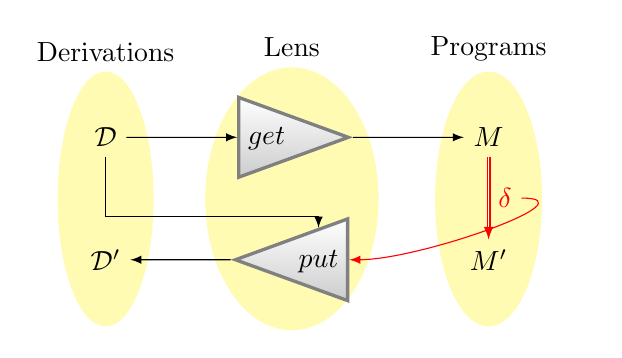
\begin{tikzpicture}[node distance=4em, auto, >=latex]
          \node (D) {$\mathcal D$}; \node (checkout) [right=of D,
          state, tribox] {$\funname{get}$}; \node (M) [right=of
          checkout] {$M$}; \node (M') [below=3em of M] {$M'$}; \node
          (commit) [state, tribox, left=of M', shape border
          rotate=180] {$\funname{put}$}; \node (D') [below=3em of D]
          {$\mathcal D'$};

          \path[->] (D) edge (checkout) (checkout) edge (M) (M) edge
          [color=red, double] node [name=delta] {$\delta$} (M')
          (commit) edge (D') ;

          \draw[->] (D) |- ++(1,-1) -| (commit) ;

          \draw[->] [out=0, in=0, color=red] (delta) edge (commit);

      \begin{pgfonlayer}{background}
        \node [fill=yellow!30,fit=(D) (D'), label=above:Derivations,
        ellipse] {}; \node [fill=yellow!30,fit=(M) (M'),
        label=above:Programs, ellipse] {}; \node
        [fill=yellow!30,fit=(checkout) (commit), label=above:Lens,
        ellipse, inner sep=0] {};
      \end{pgfonlayer}

    \end{tikzpicture}
  \end{figure}
  \begin{itemize}
  \item $\function{get}{\mathcal D}$ projects derivation $\mathcal D$
    to a program $M$
  \item $\function{put}{\mathcal D, \delta}$ checks $\delta$ against
    $\mathcal D$ and returns $\mathcal D'$
    \begin{itemize}
    \item the incremental type-checker
    \item change-based approach
    \item justification for each change ($\mathcal D'$)
    \end{itemize}
  \end{itemize}
\end{block}
\end{onlyenv}

\end{frame}

\begin{frame}[fragile]{\textcolor{greenish}{Examples}}
    \begin{center}
      \begin{tabular}{r|l}
      \textcolor{greenish}{initial term} &
      {\large\textbf{let} \textit{f x} = \textit{x} + 1
        \textbf{in} \textit{f} 3 / 2} \\[2em]\pause
      \textcolor{greenish}{easy interleave} &
      {\large\textbf{let} \textit{f x} = \alert{2 *} (\textit{x} + 1) \textbf{in}
        \textit{f} 3 / 2} \\[2em]\pause
      \textcolor{greenish}{env interleave} &
      {\large\textbf{let} \textit{f x} =
        (\alert{\textbf{let} \textit{y} = true \textbf{in}} \textit{x} + 1) \textbf{in}
        \textit{f} 3 / 2} \\[2em]\pause
      \textcolor{greenish}{type change} &
        {\large\textbf{let} \textit{f x} = \textit{x} \alert{$>$} 1
          \textbf{in} \cfbox{red}{\textit{f} 3 / 2}}
    \end{tabular}
    \end{center}
\end{frame}

\begin{frame}{In this talk...}

  \begin{onlyenv}<1>
    \begin{block}{The message}
      Generating certificates of well-typing allows type checking
      incrementality by sharing pieces of derivations
    \end{block}

  \begin{block}{The difficulty}
    Proofs are \emph{higher-order objects} (binders, substitution
    property)
    \begin{itemize}
    \item What delta language?
    \item What data structure for derivations?
    \item What language to write synthesis algorithm?
    \end{itemize}
  \end{block}
\end{onlyenv}

\begin{onlyenv}<2->
  \begin{block}{The artifact}
    \sysname{Gasp}: a \emph{language-independent} backend to develop
    certifying, incremental type checkers
    \begin{figure}
      \centering
      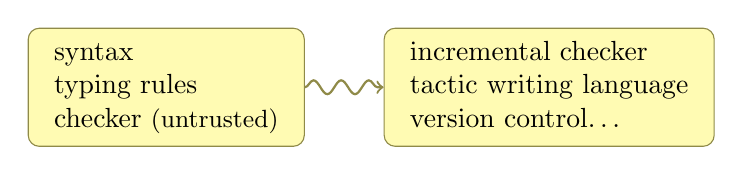
\begin{tikzpicture}
        \node[draw=yellow!50!black, fill=yellow!30, rounded corners]
        (input) {
          \begin{tabular}{l}
            syntax \\
            typing rules\\
            checker {\small (untrusted)}
          \end{tabular}
        } ;

        \node[draw=yellow!50!black, fill=yellow!30, rounded corners,
        right=of input] (output) {
          \begin{tabular}{l}
            incremental checker \\
            tactic writing language \\
            version control\ldots \\
          \end{tabular}
        } ;

        \path[->] (input) edge [draw=yellow!50!black, thick, decorate,
        decoration=snake] (output) ;
      \end{tikzpicture}
    \end{figure}
  \end{block}
  \begin{block}{The open question}
    What else can we do with it?
  \end{block}
\end{onlyenv}
\end{frame}

%%% Local Variables: 
%%% mode: latex
%%% TeX-master: "slides"
%%% End: 

% 
\begin{frame}{Certifying procedures}
  What is a certifying procedure?

  \begin{figure}
    \centering
    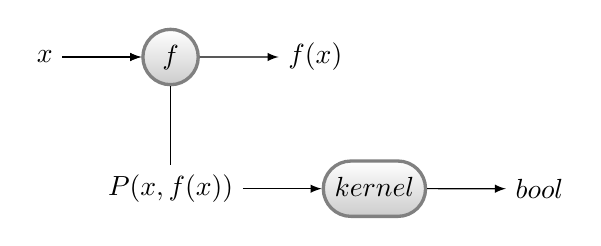
\begin{tikzpicture}[auto, >=latex]

      \node (input) {$x$};

      \node (F) [state, right=of input] {$\fct{f}$};

      \node (output) [right=of F]{$\fct{f}(x)$};

      \path[->] (input) edge (F) (F) edge (output);

      \pause

      \node (P) [below=of F]{$P(x, \fct{f}(x))$};

      \node (check) [state, right=of P] {$\fct{kernel}$};

      \node (bool) [right=of check] {$\cst{bool}$};

      \path[->]

      (input) edge (F)

      (F) [-] edge (P)

      (P) [->] edge (check)

      (check) edge (bool)

      ;

    \end{tikzpicture}
  \end{figure}

  \begin{itemize}[<3->]
  \item untrusted, complex function
  \item generic and small kernel (dB principle)
  \end{itemize}

\end{frame}

\begin{frame}{Certifying procedures}
  \begin{examples}
    \begin{itemize}
    \begin{onlyenv}<1>
    \item Theorem proving
      \begin{figure}
        \centering
        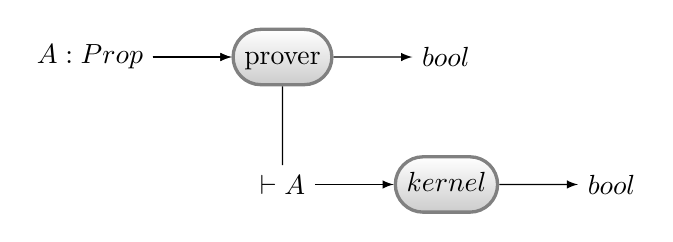
\begin{tikzpicture}[auto, >=latex]

          \node (input) {$A : \cst{Prop}$};

          \node (F) [state, right=of input] {prover};

          \node (output) [right=of F]{$\cst{bool}$};

          \path[->] (input) edge (F) (F) edge (output);

          \node (P) [below=of F]{$\vdash A$};

          \node (check) [state, right=of P] {$\fct{kernel}$};

          \node (bool) [right=of check] {$\cst{bool}$};

          \path[->]

          (input) edge (F)

          (F) [-] edge (P)

          (P) [->] edge (check)

          (check) edge (bool)

          ;

        \end{tikzpicture}
      \end{figure}
    \end{onlyenv}
      \begin{onlyenv}<2>
      \item Proof-carrying code
      \begin{figure}
        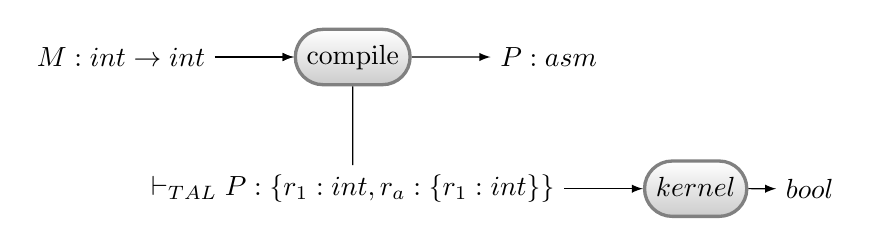
\begin{tikzpicture}[auto, >=latex]

          \node (input) {$M : \cst{int}\to\cst{int}$};

          \node (F) [state, right=of input] {compile};

          \node (output) [right=of F]{$P : \sysname{asm}$};

          \path[->] (input) edge (F) (F) edge (output);

          \node (P) [below=of F]{$\small\vdash_{\sysname{TAL}} P : \{r_1:\cst{int}, r_a:\{r_1:\cst{int}\}\}$};

          \node (check) [state, right=of P] {$\fct{kernel}$};

          \node (bool) [right=1em of check] {$\cst{bool}$};

          \path[->]

          (input) edge (F)

          (F) [-] edge (P)

          (P) [->] edge (check)

          (check) edge (bool)

          ;

        \end{tikzpicture}
\\[2em]
{\footnotesize To call $P$, the caller must place an integer in $r_1$ and a
        return label in $r_a$, the return label must accept an integer
        in $r_1$.
}      \end{figure}
    \end{onlyenv}
    \begin{onlyenv}<3>
    \item \sysname{LCF} Tactics
      \begin{figure}
        \centering
        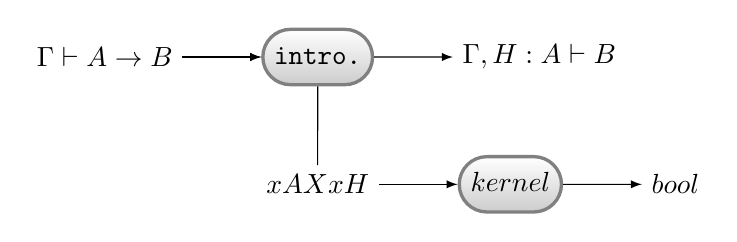
\begin{tikzpicture}[auto, >=latex]

          \node (input) {$\Gamma\vdash A\to B$};

          \node (F) [state, right=of input] {\tt intro.};

          \node (output) [right=of F]{$\Gamma, H:A\vdash B$};

          \path[->] (input) edge (F) (F) edge (output);

          \node (P) [below=of F]{$\tlam x A \smeta X {\msubst x H}$};

          \node (check) [state, right=of P] {$\fct{kernel}$};

          \node (bool) [right=of check] {$\cst{bool}$};

          \path[->]

          (input) edge (F)

          (F) [-] edge (P)

          (P) [->] edge (check)

          (check) edge (bool)

          ;

        \end{tikzpicture}
      \end{figure}
    \end{onlyenv}
    \begin{onlyenv}<4>
    \item Type checking
      \begin{figure}
        \centering
        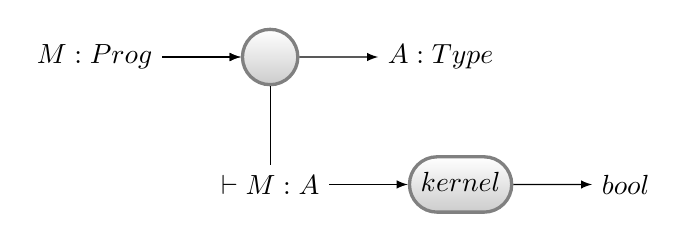
\begin{tikzpicture}[auto, >=latex]

          \node (input) {$M : \cst{Prog}$};

          \node (F) [state, right=of input] {$\finfer{}$};

          \node (output) [right=of F]{$A : \cst{Type}$};

          \path[->] (input) edge (F) (F) edge (output);

          \node (P) [below=of F]{$\vdash M : A$};

          \node (check) [state, right=of P] {$\fct{kernel}$};

          \node (bool) [right=of check] {$\cst{bool}$};

          \path[->]

          (input) edge (F)

          (F) [-] edge (P)

          (P) [->] edge (check)

          (check) edge (bool)

          ;

        \end{tikzpicture}
      \end{figure}
    \end{onlyenv}
    \end{itemize}
  \end{examples}
\end{frame}

%%% Local Variables: 
%%% mode: latex
%%% TeX-master: "slides"
%%% End: 

% \subsection{As a programmer}

\begin{frame}{\textcolor{greenish}{Example}}

  {\tt\qquad Gasp 0.1} \\[1em]

  \theprompt
  \pause
  $
  \finfer{(\recb{\s\z}{\s\z} x y {\s {\var x}})}
  $
  \\[1em]
  \pause
  $\small
  \begin{aligned}
    \md_1\ &:\ \ \vdash \s\z : \odd = \infer{\infer{ }{\vdash\z:\even}}{\vdash\s\z : \odd}\\
    \pause
    \md_2[{{\vdash x :\nat}} ]\ &: \ \ \vdash \s{\var x} : \nat =
    \infer{[\vdash x : \nat]}{\vdash \s{\var x} : \nat}\\
    \pause
    \md_3\ &:\ \ \vdash \s\z : \nat = \infer{\md_1\and \infer*{ }{\vdash
      \odd\leq\nat}}{\vdash\s\z:\nat}
    \\
    \pause
    \fbox{$\md_4$}\ &:\ \ \vdash \recb{\s\z}{\s\z} x y {\s {\var x}} :
    \nat = \infer{\md_1\and\md_3\and\infer*{[\vdash \var x:\nat]}{\md_2}}{\vdash \recb{\s\z}{\s\z} x y {\s {\var x}} :
    \nat}
  \end{aligned}
  $

  \vfill\pause
    \begin{block}{Functions}
      $\finfer{M}$ : derivation generator \\
    \end{block}
\end{frame}

\begin{frame}{\textcolor{greenish}{Example}}

  \theprompt
  \only<1>{$\finfer{(\recb{\s{\s\z}}{{\s\z}} x y {{\s {\var x}}})}$}%
  \only<2>{$\finfer{(\recb{\s{\alert{\s\z}}}{\alert{\s\z}} x y {\alert{\s {\var x}}})}$}%
  \only<3>{$\finfer{(\recb{\s{\md_1}}{\md_3} x y {\alert{\s {\var x}}})}$}%
  \only<4>{$\finfer{(\recb{\s{\fget\md_1}}{\fget\md_3} x y {\alert{\s {\var x}}})}$}%
  \only<5>{$\finfer{(\recb{\s{\fget\md_1}}{\fget\md_3} x y {\fget{\md_2}})}$}%
  \only<6->{$\finfer{(\recb{\s{\fget\md_1}}{\fget\md_3} x y {\fget{\md_2[\finfer{x}]}})}$}%

  \begin{visibleenv}<7->
    \begin{align*}
      \ldots &\ \text{(all of the above, plus:)}\\
      \md_5\ &:\ \vdash \s{\s\z}:\nat = \ldots \\
      \fbox{$\md_6$}\ &:\ \vdash \recb{\s{\s\z}}{\s\z} x y {\s{\var x}}:\nat = \ldots
    \end{align*}
  \end{visibleenv}
  \only<8->{\theprompt$\finfer{(\recb{\fget{\md_5}}{\fget{\md_3}}xy{\fget{\md_2[\md_2[\finfer{x}]]}})}$}%
  \vfill
    \begin{block}{Functions}
      $\finfer{M}$ : derivation generator \\
      \visible<4->{$\fget{\md}$ : coercion from derivation to the program it types}
    \end{block}

\end{frame}

\begin{frame}{Methodology}
  \begin{itemize}
  \item user inputs commands made of terms (programs), functions
    ($\finfer{}$, $\fget{}$) and \emph{contextual metavariables} $\md_i$
  \item to each function $A\to B$ there is an ``inverse'' $B\to A$
    (put output back into input)
  \item system evaluates functions to value (derivations)
  \item checks value (kernel)
  \item extracts (from context) and names all subterms to a map
    (repository) for future reuse: \emph{slicing}
  \end{itemize}
\end{frame}

\subsection{The \LF\ notation for derivations}

\begin{frame}{What notation for derivations?}
  \begin{onlyenv}<1-2>
    \begin{block}{Preamble}
      \begin{itemize}
      \item First-order \emph{vs.} higher-order notations
        \vspace{-2em}
        $$
        \begin{array}{ccc}
          \infer{\Gamma, A\vdash B}{\Gamma\vdash A\to B}
          &\text{\emph{vs.}}&
          \infer{[\vdash A] \\\\\vdots\\\\ \vdash B}{\vdash A\to B}
          \\\\
          \text{Explicit structural rules} &&
          \text{Handled by the notation}
        \end{array}
        $$
        \pause
      \item Local \emph{vs.} global verification
        $$
        \begin{array}{ccc}
          \infer{\infer*{\md_1}{\vdash A\to B\to C} \and \infer*{\md_2}{\vdash A}}{\vdash B\to C}
          &\text{\emph{vs.}}&
          \app M N \\[1em]
          \text{Can locally verify rule} &&
          \text{Need $M$ and $N$}
        \end{array}
        $$
      \end{itemize}
    \end{block}
  \end{onlyenv}

  \begin{onlyenv}<3>
    \begin{block}{The \LF\ notation}
      is a higher-order, local notation for derivations (and terms).\\
      Comes with a small verification algorithm (typing)
    \end{block}
    \begin{block}{Adequacy}
      \vspace{0.5em}
        \footnotesize
      \begin{tabular}{c|c|c}
        \bf in \LF, a & \bf is a & \bf example \\\hline
        atomic type constant & syntactical category & $\cst{tm} : \type$ \\
        family of types constant & judgement & $\cst{is} : \cst{tm} \to
        \cst{tp}\to\type$ \\
        object constant & constructor or rule & $\cst{lam} : (\cst{tm}\to\cst{tm})\to{\cst{tm}}$
        \\
        applied object constant & rule application &
        \\
        well-typed object & well-formed derivation &
        \\
        \hline
      \end{tabular}
    \end{block}
    \begin{examples}
      \begin{itemize}
      \item $ \text{\textsf{is\_lam}} : \prd {A,B}{\mathsf{ty}} \prd t
        {\mathsf{tm}\to \mathsf{tm}}$\quad$ (\prd x {\mathsf{tm}}
        {\textsf{is}\ x\ A} \to \textsf{is}\ (t\ x)\ B) \to
        \textsf{is}\ (\textsf{lam}\ A\ (\lam x t\ x))(\textsf{arr}\ A\
        B) $
      \item
        $\text{\textsf{is\_lam}}\ \mathsf{nat}\ \mathsf{nat}\ (\lam x
        x)\ (\lam {x h} \md[\var x, \var h])\ :\ \cst{is}\ (\cst{lam}\ \lam x {\fget\md})\
        (\cst{arr}\ \nat\ \nat) $
      \end{itemize}
    \end{examples}
  \end{onlyenv}

  \begin{onlyenv}<4->
    \begin{block}{Syntax}
      \vspace{-1.5em}
  \begin{align*}
    K &\gequal \prd x A K \gor \type &
    \text{Kind}\\
    A &\gequal \prd x A A \gor P &
    \text{Type family} \\
    P &\gequal \app {\cst a} S &
    \text{Atomic type} \\
    M &\gequal \lam x M \gor F &
    \text{Canonical object} \\
    F &\gequal \app H S &
    \text{Atomic object} \\
    H &\gequal \var x \gor \cst c &
    \text{Head}\\
    S &\gequal \spinenil \gor \spinecons M S &
    \text{Spine}\\
    % \sigma &\gequal \msubstnil \gor \msubstcons \sigma x M &
    % \text{Parallel substitution}
  \end{align*}
    \end{block}
    \begin{itemize}
    \item The $F$ are the \emph{values} we want to manipulate.
    \end{itemize}
  \end{onlyenv}
    \pause\pause\pause
    \flushright \ldots \small what are the computations?

\end{frame}

\subsection{As a type system designer}

\begin{frame}{How to write the unsafe type checker?}
  The computation language \CL:
  \begin{itemize}
  \item an unsafe language to manipulate \LF\ objects
  \item but with runtime check: each input \& output of functions must be well-typed
  \end{itemize}

  \begin{block}{Syntax}
    \vspace{-1.5em}
  \begin{align*}
    T &\gequal \lam x T \gor
    U & \text{Term} \\
    U &\gequal F \gor
    \matchin U \Gamma C & \text{Atomic term}\\
    C &\gequal \cdot \gor
    C\ \caseb P U & \text{Branches}\\
    P &\gequal \app H {\var x}\ \ldots\ {\var x} &\text{Pattern}
  \end{align*}
  \end{block}
\end{frame}

\begin{frame}{\textcolor{greenish}{Example}}
  \begin{onlyenv}<1-3>
    \begin{mathleft}
      \finfer{}\ :\ \prd M {\cst{tm}} \sig A {\cst{tp}} (\vdash M : A)
      =
      \\
      \pause
      \lamd M \match{M} \\
      \pause
      \quad\caseb{\z} \pair {\cst{even}}{\infer{ }{\vdash \cst o : \cst{even}}} \\
      \quad\caseb{\s M}
      \match{\finfer M} \\
      \quad\quad\caseb{\pair{\cst{even}}\md}
      \pair {\cst{odd}}{\infer\md{\vdash\app{\cst{s}} M : \cst{odd}}} \\
      \quad\quad\caseb{\pair{\cst{odd}}\md}
      \pair {\cst{even}}{\infer\md{\vdash\app{\cst{s}} M : \cst{even}}} \\
      \quad\quad\caseb{\pair{\cst{nat}}\md}
      \pair {\cst{nat}}{\infer\md{\vdash\app{\cst{s}} M : \cst{nat}}} \\
    \end{mathleft}
  \end{onlyenv}

  \begin{onlyenv}<4>
    \begin{mathleft}
  \quad\caseb{\app{M}N} \\
  \quad\quad\letd {\pair {A_1\to B} {\md_1}} {\finfer{M}} \\
  \quad\quad\letd {\pair {A_2} {\md_2}} {\finfer{N}} \\
  \quad\quad\letd {\md_{\leq}} {\fleq {A_1} {A_2}} \\
  \quad\quad
  \match{\md_{\leq}} \\
  \quad\quad\quad\caseb{\infer{ }{\vdash A\leq A}}
  \pair {B} {\infer{\md_1 \and \md_2}{\vdash \app M N : B}} \\
  \quad\quad\quad\caseb{\_}
  \pair {B} {\infer{\md_1 \and \infer*{\md_2 \and \md_{\leq}}{\vdash N
      : A_1}}{\vdash \app M N : B}}
    \end{mathleft}

    \begin{block}{Functions}
      $\fleq{}{}\ :\ \prd A
      {\cst{tp}} \prd B {\cst{tp}} \vdash A\leq B = \ldots$
    \end{block}
  \end{onlyenv}

  % lambda
  \begin{onlyenv}<5-8>
    \begin{mathleft}
      \quad\caseb{\tlam x A M}
      \uncover<6->{
        \\\quad\quad
        \syntax{let}{\pair B \md}
        \only<8->{\syntax{in}{\env {$\md_{\var x}$}{(\vdash {\var x} : A)}}}
        \syntax{=}
        \\\quad\quad\quad
        {\finfer {\alt<-6> M {\gsubst M {\msubst x {\fget{\pair A {\md_{\var
                      x}}}}}}}}
        \syntax{in}
        \\\quad\quad
        \pair {A\to B}
        {\infer{
            \mbox{$      \begin{array}{c}
                \uncover<7->{{[\md_{\var x}]} \\}
                {\md}
              \end{array}
              $}    }{
            \vdash\lam x M : A\to B
          }}
      }      \\[2em]
      \quad\text{\only<7->\sout{$\caseb{\var x}\ \uncover<6->{???}$}}
    \end{mathleft}
    \uncover<7->{
      \begin{block}{Note}
        $\finfer{\fget{\pair{A}{\md}}} = \pair{A}{\md}$
      \end{block}
    }
  \end{onlyenv}

  \begin{onlyenv}<9->
    \begin{mathleft}
  \quad\caseb{\recb M N x y P} \\
  \quad\quad
  \letd {\pair {A_M} {\md_M}} {\finfer{M}} \\
  \quad\quad
  \letd {\md_{A_M}} {{A_M} \leq \cst{nat}} \\
  \quad\quad
  \letd {\pair {A_N} {\md_N}} {\finfer{N}} \\
  \quad\quad
  \syntax{let} {\pair {A_P} {\md_P}} \syntax{in}
  {(\envcons {\env {$\md_x$} {(\vdash
        \var x : \cst{nat})}} {$\md_y$} {(\vdash\var y : A_N)})} = \\
  \quad\quad\quad
  {\finfer{\gsubst P {\msubstcons {\msubst x
          {\fget{\pair{\cst{nat}}{\md_x}}}} y
        {\fget{\pair{A_N}{\md_y}}}}}} \syntax{in}\\
  \quad\quad\letd {\pair A {\pair{\md_{A_N}}{\md_{A_P}}}} {{A_N} \sqcap {A_P}} \\
  \quad\quad
  \syntax{let} {\pair {\_} {\md_P}} \syntax{in}
  {(\envcons {\env {$\md_x$} {(\vdash
        \var x : \cst{nat})}} {$\md_y$} {(\vdash\var y : A)})} = \\
  \quad\quad\quad
  {\finfer{\gsubst P {\msubstcons {\msubst x
          {\fget{\pair{\cst{nat}}{\md_x}}}} y
        {\fget{\pair{A}{\md_y}}}}}} \syntax{in}\\
  \quad\quad\pair {A} {
    \infer{
      \infer*{\md_M \and \md_{A_M}}
      {\vdash M : A} \and
      \infer*{\md_N \and \md_{A_N}}
      {\vdash N : A}\and
      \infer*{\infer*{}{\mbox{$
        \begin{array}{c}
          [\md_x] [\md_y] \\
          \md_P
      \end{array}
        $}} \and \md_{A_P}}{\vdash P : A}
    }{
      \vdash \recb M N x y P : A
    }
  }
    \end{mathleft}
    \begin{block}{Functions}
      $\sqcap\ :\ \prd{A}{\cst{tp}} \prd{B}{\cst{tp}} \sig C {\cst{tp}}
      (\vdash A\leq C )\times(\vdash B\leq C) = \ldots$
    \end{block}
  \end{onlyenv}

\end{frame}

\begin{frame}{Discussion}
  \begin{itemize}[<+->]
  \item the ``type'' of a function is a kind of \emph{contract}:
    \begin{figure}
      \centering
      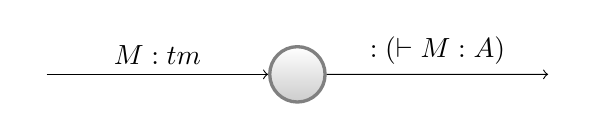
\begin{tikzpicture}[auto]
        \node (in) {}; \node (F) [state, right=8em of in] {$\finfer{}$};
        \node (out) [right=8em of F]{};

        \path[->] (in) edge node (m) {$M : \cst{tm}$} (F) (F) edge
        node (d)
        {$\md : (\vdash M : A)$} (out);
      \end{tikzpicture}
    \end{figure}
  \item ``inverses'' used to feed output back to input, same idea as
    \emph{context-free} typing:

    $$M \gequal \var x \gor \app M M \gor \tlam x A M \gor \{\var x :
    A\} $$
    \begin{mathpar}
      \infer{ \vdash \gsubst M {\msubst x {\{\var x:A\}}} : B }{ \vdash
        \tlam x A M : A\to B }

      \infer{ }{ \vdash \{\var x : A\} : A }
    \end{mathpar}

  \end{itemize}
  
\end{frame}

%%% Local Variables: 
%%% mode: latex
%%% TeX-master: "slides"
%%% End: 

% 
\subsection{Data structures}

\begin{frame}{Sliced \LF}
  \begin{block}{Syntax}
  \begin{align*}
    K &\gequal \prd x A K \gor \type &
    \text{Kind}\\
    A &\gequal \prd x A A \gor P &
    \text{Type family} \\
    P &\gequal \app {\cst a} S &
    \text{Atomic type} \\
    M &\gequal \lam x M \gor F &
    \text{Canonical object} \\
    F &\gequal \app H S \gor \alert{\smeta X \sigma} &
    \text{Atomic object} \\
    H &\gequal \var x \gor \cst c \gor \alert{\fct{f}} &
    \text{Head}\\
    S &\gequal \spinenil \gor \spinecons M S &
    \text{Spine}\\
    \sigma &\gequal \msubstnil \gor \msubstcons \sigma x M &
    \text{Parallel substitution}
  \end{align*}
  \vspace{-1.5em}
  \begin{itemize}
    \item The $\smeta X \sigma$ stand for open objects (CMTT).
    \item The $\sigma$ close them.
    \item The $\fct{f}$ are computations to do
  \end{itemize}
  \end{block}
\end{frame}

\begin{frame}[fragile]{Data structures}
  \begin{block}{Signature}
    An object language is defined by a \emph{signature}:
    \begin{align*}
      \Sigma &\gequal \gnil \gor \gcons \Sigma {\cst a : K} \gor \gcons
      \Sigma {\cst c : A} \gor \alert{\gcons \Sigma {\fct f : A = T}}
    \end{align*}
  \end{block}
  \begin{block}{Repository}
    A \emph{repository} is the sliced representation of an atomic object (\verb'evar_map'):
    $$ \mr\;:\;(\meta X \mapsto (\Gamma\vdash\tp F P))\times\smeta X
    \sigma $$

    We define $\checkout{\mr}$ the operation of stripping out all metavariables
  \end{block}
\end{frame}

\begin{frame}{Inverse functions}
  To each $\fct{f}:A=T\in\Sigma$, associate a family of $\fcti{f} n
  : A^{-n} = T^{-n}$\\
  Project out the $n$-th argument of $\fct{f}$
  \begin{examples}
    \begin{itemize}
    \item
      $\fct{infer} : \prd M {\cst{tm}} \sig A {\cst{tp}}
      {\app{\cst{is}}\app M A}  = T$ \\
      $\fcti{infer}{0} : \prd {\{M\}} {\cst{tm}}
      {(\sig A {\cst{tp}}
      {\app{\cst{is}}\app M A})} \to \cst{tm} = \lam x \lam y \var x$

    \item $\fct{equal} : \prd M {\cst{tm}} \prd N {\cst{tm}}
      \app{\cst{eq}}\app M N = T'$\\
      $\fcti{equal}{0} : \prd {\{M\}} {\cst{tm}} \prd {\{N\}}
      {\cst{tm}} \app{\cst{eq}}\app M N \to \cst{tm} = \lam m \lam n
      \lam h \var m $  \\
      $\fcti{equal}{1} : \prd {\{M\}} {\cst{tm}} \prd {\{N\}}
      {\cst{tm}} \app{\cst{eq}}\app M N \to \cst{tm} = \lam m \lam n
      \lam h \var n $  \\
    \end{itemize}
  \end{examples}
  \begin{block}{Evaluation}
    \begin{itemize}
    \item $\fct{infer}\ (\fcti{infer} 0 \pair A \md) = \pair A \md$
    \item $\fct{equal}\ (\fcti{equal} 0\ \md)\ (\fcti{equal} 1\ \md) = \md$
    \end{itemize}
  \end{block}
\end{frame}

\subsection{Typed evaluation algorithm}

\begin{frame}{The typed evaluation algorithm}
  In \textcolor{blue}{[P. \& R-G., CPP'12]}, we define $\commit \mr F$:
  \begin{itemize}
  \item evaluates functions $\fct f$ in $F$
  \item checks $F$, functions arguments and return (\wrt\ type of
    $\fct f$)
  \item slices values in $\mr$
  \item returns the enlarged $\mmr$
  \end{itemize}
\end{frame}

\begin{frame}{Evaluation strategy}
  \begin{itemize}[<+->]
  \item We want strong reduction\\
    \textcolor{greenish}{Example}\quad
    $\cst{lam}\ \lam x \alert{\fct{f}\ (\s {\var x})} $
    {\footnotesize not a value}
  \item But not call-by-value\\
    \textcolor{greenish}{Example}\quad
    $\finfer{(\recb{\s{\alert{\fget\md_1}}}{\fget\md_3} x y {\fget{\md_2[\alert{\finfer{x}}]}})}$
  \item And not call-by-name either \\
    \textcolor{greenish}{Example}\quad
    $\finfer{(\alert{\fct{id}}\ (\fget{\md}))}${\footnotesize$\neq\md$}
  \end{itemize}
  \pause
  \begin{block}{Ugly solution}
    Strong call-by-name \emph{except} in function argument position\\
    \qquad$\leadsto$ weak head call-by-name
  \end{block}
\end{frame}

\begin{frame}{Conclusion}
  \begin{center}
    \huge Demo
  \end{center}
\end{frame}

%%% Local Variables: 
%%% mode: latex
%%% TeX-master: "slides"
%%% End: 



\end{document}
